\section{Task 3: Approximate Bayesian Computation (ABC)}
\label{sec:task3}

Least squares gives one best value for each parameter. A Bayesian approach instead gives a full posterior distribution, which shows which values are plausible and how the parameters depend on each other. Rejection ABC approximates the posterior without writing down the likelihood: it only needs to simulate model output and compare it with the data \citep{beaumont2002,sunnaker2013}. The code is in Appendix~\ref{app:task3}.

\subsection{Task 3.1: Choice of parameters}
The Model~2 estimates were ranked by absolute value with R's \texttt{order()} function (Appendix~\ref{app:task3}, ``Task 3.1''). The two largest are $\theta_{bias}=120.022$ and $\theta_1=4.4805$ (the $x_4$ coefficient), so these two were estimated with ABC. The other two were fixed at their least squares values, $\theta_2=1.20018$ ($x_1^3$) and $\theta_3=0.800003$ ($x_3^4$).

\subsection{Task 3.2: Uniform priors}
A uniform prior was placed around each least squares estimate. To set a sensible width, the standard errors of the estimates were computed from $\hat\sigma^2(\mathbf{X}^T\mathbf{X})^{-1}$: $\text{SE}(\theta_{bias})=0.0978$ and $\text{SE}(\theta_1)=0.0167$. Each prior was set to the estimate $\pm10$ standard errors:
\begin{align*}
\theta_{bias}&\sim U(119.045,\;121.000),\\
\theta_1&\sim U(4.3135,\;4.6475).
\end{align*}
This range is wide enough to cover all plausible values, since the true value lies within a few standard errors of the estimate. It is also narrow enough that a useful share of the draws is accepted. A prior of $\pm50\%$ of the estimate would accept almost nothing, because these parameters are known so precisely.

\subsection{Task 3.3: Rejection ABC}
The algorithm used was:
\begin{enumerate}
  \item Draw $N=100{,}000$ pairs $(\theta_{bias}^{(j)},\theta_1^{(j)})$ independently from the two uniform priors, with the random seed fixed at 456 so that the run can be repeated.
  \item For each pair, compute the model output, with $\theta_2,\theta_3$ fixed:
  \[\hat{\mathbf y}^{(j)}=\theta_{bias}^{(j)}+\theta_1^{(j)}x_4+\theta_2x_1^3+\theta_3x_3^4.\]
  \item Measure the distance from the data as $\text{RSS}^{(j)}=\sum_i(y_i-\hat y_i^{(j)})^2$.
  \item Accept the pair if $\text{RSS}^{(j)}\le\epsilon$, with $\epsilon=1.0005\times\text{RSS}_{LS}=250935.9$, that is, if it fits within 0.05\% of the best possible fit.
\end{enumerate}
The tolerance allows the RSS to rise by 125.4, which is about $5\hat\sigma^2$, or a drop of about 2.5 in the log-likelihood. A tolerance on this scale keeps parameter values that are statistically compatible with the data. The RSS of the prior draws ranged from 250{,}811 to 275{,}113. In total, \textbf{1921 draws were accepted} (an acceptance rate of 1.92\%), enough for stable histograms.

\subsection{Task 3.4: Joint and marginal posterior distributions}
Figure~\ref{fig:abc} shows the accepted samples. The left panel is the joint posterior and the other two panels are the marginal posteriors. The red markers show the least squares estimates. Table~\ref{tab:abc} summarises the posteriors.

\begin{figure}[H]
\centering
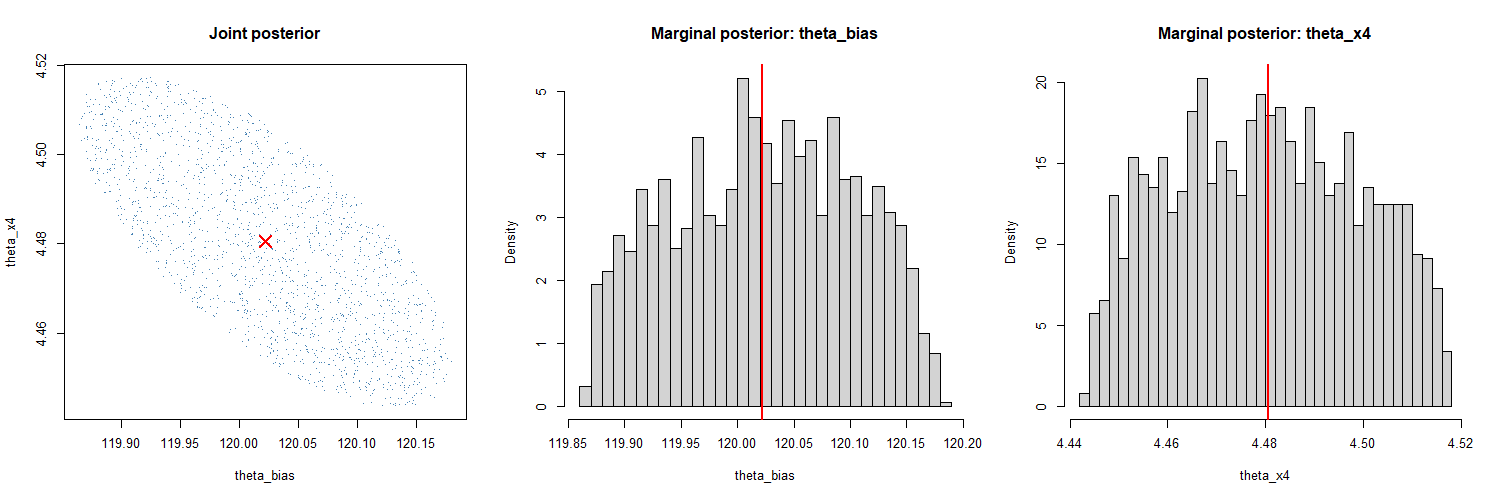
\includegraphics[width=\textwidth]{fig7_abc_posterior.png}
\caption{Rejection ABC results for Model~2: joint posterior of $(\theta_{bias},\theta_{x_4})$ (left) and marginal posteriors (centre, right). The red markers show the least squares estimates.}
\label{fig:abc}
\end{figure}

\begin{table}[H]
\centering
\caption{Posterior summaries from 1921 accepted ABC samples.}
\label{tab:abc}
\small
\begin{tabular}{lccccc}
\toprule
Parameter & LS est. & Post.\ mean & Post.\ SD & 95\% cred.\ interval & Prior range \\
\midrule
$\theta_{bias}$ & 120.022 & 120.023 & 0.079 & [119.881, 120.157] & [119.045, 121.000] \\
$\theta_1$ ($x_4$) & 4.4805 & 4.4799 & 0.019 & [4.4479, 4.5134] & [4.3135, 4.6475] \\
\bottomrule
\end{tabular}
\end{table}

\subsection{Task 3.5: Explanation of the results}
\textbf{Agreement with least squares.} Both posterior means agree with the least squares estimates to three or four significant figures, and both estimates lie in the centre of the joint cloud. This is expected: with a flat prior, the posterior is driven by the likelihood, and least squares is the maximum likelihood estimate.

\textbf{Learning from the data.} The posterior ranges are much narrower than the priors. The 95\% credible interval of $\theta_{bias}$ (width 0.28) covers only about 14\% of the prior width of 1.96, and that of $\theta_1$ (width 0.066) about 20\% of the prior width of 0.33. The data have greatly reduced the uncertainty. Both intervals exclude zero by a wide margin, so network traffic has a clear positive effect on power ($\approx4.5$\,W per unit of $x_4$), even though Task~1 showed almost no correlation between $x_4$ and $y$ on its own. The idle power is about 120\,W.

\textbf{Correlation between parameters.} The joint posterior is a tilted ellipse with correlation $-0.71$. Network traffic is always positive (mean 3.0), so a larger $\theta_1$ raises every prediction by about $3\,\Delta\theta_1$. A smaller intercept can cancel this. The data cannot fully separate the two effects, so they trade off against each other. This information is lost if the parameters are reported one at a time.

\textbf{Shape of the posterior.} The marginal histograms are rounded and fairly flat on top rather than bell-shaped. This comes from the method. A fixed RSS threshold accepts every draw inside an ellipse of nearly equal fit, and because the prior is uniform, the accepted points are spread almost evenly inside that ellipse. A smaller tolerance (with more draws), or a version that adds simulated Gaussian noise to each output, would give a shape closer to the true Gaussian posterior. The location, spread and correlation would stay much the same.
